\documentclass[xcolor=dvipsnames, 11pt]{beamer}
\usetheme{AnnArbor}

\usecolortheme{crane}
\setbeamertemplate{caption}[numbered]
\usepackage{float}
\usepackage{graphicx}
\usepackage{subcaption}
\graphicspath{{./ripser/}}
\usepackage[utf8]{inputenc}
\usepackage{amsmath}
%\usepackage{tabto}
\usepackage{amsfonts}
\usepackage{amssymb}
\usepackage{amsthm}
\usepackage{mathtools}
\usepackage{stmaryrd}
\usepackage{xcolor}
\usepackage{pst-solides3d}
\usepackage{tikz}
\usepackage{tikz-3dplot}
\usepackage{pgfplots}
\usepackage{tkz-fct}
\usepackage{tikz-cd}
\usepackage[affil-it]{authblk}
\usepackage{tkz-euclide}
\usetikzlibrary{decorations.markings,shapes.misc,arrows.meta,shapes.geometric,intersections}
\usepackage{cancel}

\usepackage[all,knot,arc,poly]{xy}
\let\amsamp=&

% 
%\setlength{\topmargin}{30mm}
%\addtolength{\topmargin}{-1in}
%\addtolength{\topmargin}{-\headsep}
%\addtolength{\topmargin}{-\headheight}
%\addtolength{\topmargin}{-\topskip}

%\setlength{\textheight}{270mm}
%\addtolength{\textheight}{\topskip}
%\addtolength{\textheight}{-\footskip}
%\addtolength{\textheight}{-30pt}

%\setlength{\oddsidemargin}{-1in}
%\addtolength{\oddsidemargin}{20mm}
%\setlength{\evensidemargin}{\oddsidemargin}

%\setlength{\textwidth}{170mm}

\newtheorem{defn}{Definition}[section]
 \newtheorem{thm}{Theorem}[section]
 \newtheorem{Lemma}{Lemma}[section]
 \newtheorem{Claim}{Claim}[section]
 \newtheorem{Prop}{Proposition}[section]
  \theoremstyle{definition}\newtheorem{Ex}{Example}[section]
 \newtheorem{Cor}{Corollary}[section]
 \newtheorem{claim}{Claim}[section]
 \newtheorem{conj}{Conjecture}  

\usepackage {amsfonts,amssymb}
%\usepackage{mathbbol}
\usepackage{latexsym}
\usepackage{mathrsfs}
\input xy
\xyoption{all}

\newcommand {\op}{\mathcal{O}\mathfrak{p}}
\newcommand {\Def}{\textrm{Def}}
\newcommand {\MC} {\textrm{MC}}
\newcommand {\Art}{\textrm{Art}_\CC}
\newcommand {\Kur}{\textrm{Kur}}
\newcommand {\LG} {^LG}
\newcommand{\fart}{\textrm{FArt}_\CC}
\newcommand{\fun}{\textrm{Fun}}
\newcommand{\sets}{\textrm{Sets}}
\newcommand{\tops}{\textrm{Top}}

\newcommand {\BB}{\mathbb{B}}
\newcommand {\CC}{\mathbb{C}}
\newcommand {\FF}{\mathbb{F}}
\newcommand {\KK}{\mathbb{K}}
\newcommand {\MM}{\mathbb{M}}
\newcommand{\NN}{\mathbb{N}}
\newcommand {\PP}{\mathbb{P}}
\newcommand{\QQ}{\mathbb{Q}}
\newcommand {\RR}{\mathbb{R}}
\newcommand {\SSS}{\mathbb{S}}
\newcommand {\VV}{\mathbb{V}}
\newcommand {\HH}{\mathbb{H}}
\newcommand {\WW}{\mathbb{W}}
\newcommand{\YY}{\mathbb{Y}}
\newcommand{\ZZ}{\mathbb{Z}}


\newcommand {\bal}{\boldsymbol{\alpha}}
\newcommand {\bbe}{\boldsymbol{\beta}}
\newcommand {\bga}{\boldsymbol{\gamma}}
\newcommand {\bmu}{\boldsymbol{\mu}}
\newcommand {\bom}{\boldsymbol{\omega}}
\newcommand {\bth}{\boldsymbol{\theta}}
\newcommand {\bph}{\boldsymbol{\phi}}
\newcommand {\bdh}{\boldsymbol{h}}
\newcommand {\bdk}{\boldsymbol{k}}
\newcommand {\bdE}{\boldsymbol{E}}
\newcommand {\bdU}{\boldsymbol{U}}
\newcommand {\bdP}{\boldsymbol{P}}
\newcommand {\ba}{{\bf a}}
\newcommand {\bb}{{\bf b}}
\newcommand {\bc}{{\bf c}}
\newcommand {\bd}{{\bf d}}
\newcommand {\bg}{{\bf g}}
\newcommand {\be}{{\bf e}}
\newcommand {\bdf}{{\bf f}}
\newcommand {\bp}{{\bf p}}
\newcommand {\bq}{{\bf q}}
\newcommand {\bv}{{\bf v}}
\newcommand {\bh}{{\bf h}}
\newcommand {\bk}{{\bf k}}
\newcommand {\br}{{\bf r}}
\newcommand {\bdu}{{\bf u}}
\newcommand {\bdv}{{\bf v}}
\newcommand {\bi}{{\bf i}}
\newcommand {\bj}{{\bf j}}
\newcommand {\bn}{{\bf n}}
\newcommand {\bs}{{\bf s}}
\newcommand {\bt}{{\bf t}}
\newcommand {\bu}{{\bf u}}
\newcommand {\bw}{{\bf w}}
\newcommand {\bx}{{\bf x}}
\newcommand{\by}{{\bf y}}
\newcommand {\bz}{{\bf z}}
\newcommand {\bB}{{\bf B}}
\newcommand{\bD}{{\bf D}}
\newcommand {\bE}{{\bf E}}
\newcommand {\bF}{{\bf F}}
\newcommand {\bG}{{\bf G}}
\newcommand {\bH}{{\bf H}}
\newcommand {\bK}{{\bf K}}
\newcommand {\bL}{{\bf L}}
\newcommand {\bM}{{\bf M}}
\newcommand {\bN}{{\bf N}}
\newcommand {\bO}{{\bf O}}
\newcommand {\bP}{{\bf P}}
\newcommand {\bQ}{{\bf Q}}
\newcommand {\bR}{{\bf R}}
\newcommand {\bT}{{\bf T}}
\newcommand {\bS}{{\bf S}}
\newcommand {\bU}{{\bf U}}
\newcommand {\bV}{{\bf V}}
\newcommand {\bW}{{\bf W}}
\newcommand {\bgamma}{\boldsymbol\gamma}
\newcommand {\bdelta}{\boldsymbol\delta}
\newcommand {\bDelta}{\boldsymbol\Delta}
%\newcommand{\qed}{{\ \bf qed}}

\newcommand {\rroot}{\mathbf{root}}
\newcommand {\coroot}{\mathbf{coroot}}
\newcommand {\weight}{\mathbf{weight}}
\newcommand {\coweight}{\mathbf{coweight}}
 \newcommand{\higgs}{\textrm{Higgs}}
\newcommand{\bun}{\textrm{Bun}}
\newcommand{\rk}{\textrm{rk}}
\newcommand{\ext}{\textrm{Ext}}
% \newcommand {\id}{\mathbb{1}}
% Use \id if using mathbbol instead of amssymb
\newcommand{\range}{\textrm{Range}}
\newcommand{\arccot}{\textrm{arccot}}

\newcommand{\thickslash}{\mathbin{\!\!\pmb{\fatslash}}}


\newcommand{\cA}{\mathcal{A}}
\newcommand{\cB}{\mathcal{B}}
\newcommand{\cC}{\mathcal{C}}
\newcommand{\cD}{\mathcal{D}}
\newcommand{\cE}{\mathcal{E}}
\newcommand{\cF}{\mathcal{F}}
\newcommand{\cG}{\mathcal{G}}
\newcommand{\cH}{\mathcal{H}}
\newcommand{\cI}{\mathcal{I}}
\newcommand{\cJ}{\mathcal{J}}
\newcommand{\cK}{\mathcal{K}}
\newcommand{\cL}{\mathcal{L}}
\newcommand {\cM}{\mathcal{M}}
\newcommand {\cN}{\mathcal{N}}
\newcommand {\cO}{\mathcal{O}}
\newcommand{\cP}{\mathcal{P}}
\newcommand{\cQ}{\mathcal{Q}}
\newcommand{\cR}{\mathcal{R}}
\newcommand{\cS}{\mathcal{S}}
\newcommand{\cT}{\mathcal{T}}
\newcommand{\cU}{\mathcal{U}}
\newcommand{\cV}{\mathcal{V}}
\newcommand{\cW}{\mathcal{W}}
\newcommand{\cX}{\mathcal{X}}
\newcommand{\cY}{\mathcal{Y}}
\newcommand{\cZ}{\mathcal{Z}}

\newcommand{\loc}{\mathcal{L}oc}
\newcommand{\Loc}{\textrm{Loc}}
\newcommand{\cih}{\mathpzc{h}}
\newcommand{\cx}{\mathpzc{x}}
\newcommand{\cy}{\mathpzc{y}}
\newcommand{\ce}{\mathpzc{e}}
\newcommand{\cf}{\mathpzc{f}}
\newcommand{\cl}{\mathpzc{l}}




 




\newcommand{\scA}{\mathscr{A}}
\newcommand{\scB}{\mathscr{B}}
\newcommand{\scC}{\mathscr{C}}
\newcommand{\scD}{\mathscr{D}}
\newcommand{\scE}{\mathscr{E}}
\newcommand{\scF}{\mathscr{F}}
\newcommand{\scG}{\mathscr{G}}
\newcommand{\scH}{\mathscr{H}}
\newcommand{\scI}{\mathscr{I}}
\newcommand{\scJ}{\mathscr{J}}
\newcommand{\scK}{\mathscr{K}}
\newcommand{\scL}{\mathscr{L}}
\newcommand{\scM}{\mathscr{M}}
\newcommand{\scP}{\mathscr{P}}
\newcommand{\scR}{\mathscr{R}}
\newcommand{\scO}{\mathscr{O}}
\newcommand{\scS}{\mathscr{S}}
\newcommand{\scT}{\mathscr{T}}
\newcommand{\scU}{\mathscr{U}}
\newcommand{\scV}{\mathscr{V}}
\newcommand{\scW}{\mathscr{W}}
\newcommand{\scX}{\mathscr{X}}
\newcommand{\scY}{\mathscr{Y}}
\newcommand{\scZ}{\scZ}

\newcommand{\uR}{\underline{\mathbb{R}}}
\newcommand {\uC}{\underline{\mathbb{C}}}


\newcommand{\fh}{\mathfrak{h}}
\newcommand{\fa}{\mathfrak{a}}
\newcommand{\fb}{\mathfrak{b}}
\newcommand{\fc}{\mathfrak{c}}
\newcommand{\fg}{\mathfrak{g}}
\newcommand{\fk}{\mathfrak{k}}
\newcommand{\fl}{\mathfrak{l}}
\newcommand{\fm}{\mathfrak{m}}
\newcommand{\fn}{\mathfrak{n}}
\newcommand{\fo}{\mathfrak{o}}
\newcommand{\fp}{\mathfrak{p}}
\newcommand{\fr}{\mathfrak{r}}
\newcommand{\fs}{\mathfrak{s}}
\newcommand{\fsu}{\mathfrak{su}}
\newcommand{\ft}{\mathfrak{t}}
\newcommand{\slt}{\mathfrak{sl}_2(\CC)}
\newcommand{\sln}{\mathfrak{sl}(n)}
\newcommand{\fsl}{\mathfrak{sl}}
\newcommand{\fu}{\mathfrak{u}}
\newcommand{\fv}{\mathfrak{v}}
\newcommand{\fx}{\mathfrak{x}}
\newcommand{\fy}{\mathfrak{y}}
\newcommand{\fz}{\mathfrak{z}}
\newcommand{\fA}{\mathfrak{A}}
\newcommand{\fB}{\mathfrak{B}}
\newcommand{\fD}{\mathfrak{D}}
\newcommand{\fM}{\mathfrak{M}}
\newcommand{\fR}{\mathfrak{R}}
\newcommand {\fU}{\mathfrak{U}}
\newcommand {\fV}{\mathfrak{V}}
\newcommand {\fW}{\mathfrak{W}}
\newcommand{\fX}{\mathfrak{X}}
\newcommand{\faff}{\mathfrak{aff}}

\newcommand{\Aff}{\textrm{Aff}}

\newcommand{\sym}{\textrm{Sym}}

\newcommand {\dbar}{\overline{\partial}}
\newcommand {\zbar}{\overline{z}}
\newcommand {\zvec}{\underline{z}}
\newcommand {\dzbar}{d\overline{z}}
\newcommand {\Nbar}{\overline{N}}
\newcommand {\Kbar}{\overline{K}}
\newcommand{\diff}{\textrm{Diff}}

%\newcommand {\hom}{\textrm{Hom}}

\newcommand{\mhom}{\textrm{Hom}}
\newcommand {\mend}{\textrm{End}}
\newcommand {\misom}{\textrm{Isom}}
\newcommand {\maut}{\textrm{Aut}}
\newcommand{\pr}{\textrm{pr}}

\newcommand {\sisom}{\underline{Isom}}
\newcommand {\saut}{\underline{Aut}}
\newcommand {\shom}{\textrm{\underline{Hom}}}
\newcommand {\send}{\underline{End} }

\newcommand{\dra}{M^{an}_{DR}(X,G)}
\newcommand{\dr}{M_{DR}(X,G)}

\newcommand {\ad}{\textrm{ad} }
\newcommand{\Ad}{\textrm{Ad}}

\newcommand{\lspan}{\textrm{span}}
\newcommand{\img}{\textrm{Im }}
\newcommand{\spec}{\textrm{Spec }}
\newcommand{\specan}{\textrm{Spec}^{an}}
\newcommand{\gspec}{\underline{\textrm{Spec }}}
\newcommand {\cok}{\textrm{coker}}
\newcommand{\tot}{\textrm{tot }}
\newcommand{\tildel}{\widetilde{\delta}}
\newcommand{\ctimes}{\otimes_\CC}
\newcommand{\sotimes}{\otimes_{\cO_X}}
\newcommand{\pic}{\textrm{Pic}}
\newcommand{\tr}{\textrm{tr }}

\newcommand  {\eps}{\varepsilon}
\newcommand {\kap}{\varkappa}
\newcommand {\io}{\iota}
\newcommand {\fii}{\varphi}

\newcommand{\Higgs}{{\bf Higgs}}
\newcommand{\Bun}{{\bf Bun}}
\newcommand{\gHiggs}{\op{\boldsymbol{\mathcal{H}iggs}}}
\newcommand{\Prym}{{\bf Prym}}
\newcommand{\Jac}{{\bf Jac}}
%\newcommand{\bh}{\boldsymbol{h}}
%\newcommand{\bH}{\boldsymbol{\mathcal{H}}}
\newcommand{\rts}{{\sf root}}
\newcommand{\wts}{{\sf weight}}
\newcommand{\crts}{{\sf coroot}}
\newcommand{\cwts}{{\sf coweight}}
\newcommand{\chr}{{\sf char}}
\newcommand{\cchr}{{\sf cochar}}

\newcommand{\Aut}{\textrm{Aut}}
\newcommand{\Der}{\textrm{Der}}
\newcommand{\spin}{\textrm{Spin}}
\newcommand{\spinc}{\textrm{Spin}^c}
%\newcommand{\U}{\boldsymbol{U(1)}}

\newcommand{\Mat}{\textrm{Mat}}

\newcommand{\hookr}{\hookrightarrow}

%%%%%%%%%%%%%%%%%%%%%%%%%%%%%%%%%%%%%%%%%%%%%%%%%%%%%%%%%%%%%%%%%%%%%%%%%
% Long exact sequence macro
%%%%%%%%%%%%%%%%%%%%%%%%%%%%%%%%%%%%%%%%%%%%%%%%%%%%%%%%%%%%%%%%%%%%%%%%%

\newcommand{\les}[9]{
\xymatrix{
 0 \ar[r] & {#1} \ar[r]  &  {#2} \ar[r]  &  {#3}
\ar@{->}`r/10pt[d] `[l] `^dl[dlll]  `^dr/10pt[dll]    [dll] \\
 &  {#4} \ar[r] & {#5} \ar[r] & {#6}
\ar@{->}`r/10pt[d] `[l] `^dl[dlll]  `^dr/10pt[dll]    [dll] \\
 & {#7} \ar[r]  & {#8} \ar[r] & {#9}
\ar@{->}`r/10pt[d] `[l] `^dl[dlll]  `^dr/10pt[dll]    [dll] \\
 & 0 \ar[r] & \cdots & }
}


%%%%%%%%%%%%%%%%%%%%%%%%%%%%%%%%%%%%%%%%%%%%%%%%%%%%%%%%%%%%%%%%%%%%%%%%%

\newcommand{\lestwo}[9]{
\xymatrix{     
 0 \ar[r] & {#1} \ar[r]  &  {#2} \ar[r]  &  {#3} 
\ar@{->}`r/10pt[d] `[l] `^dl[dlll]  `^dr/10pt[dll]    [dll] \\
 &  {#4} \ar[r] & {#5} \ar[r] & {#6} 
\ar@{->}`r/10pt[d] `[l] `^dl[dlll]  `^dr/10pt[dll]    [dll] \\
 & {#7} \ar[r]  & {#8} \ar[r] & {#9} }
}

%%%%%%%%%%%%%%%%%%%%%%%%%%%%%%%%%%%%%%%%%%%%%%%%%%%%%%%%%%%%%%%%%%%%%%%%%
% Long exact sequence macro
%%%%%%%%%%%%%%%%%%%%%%%%%%%%%%%%%%%%%%%%%%%%%%%%%%%%%%%%%%%%%%%%%%%%%%%%%

\newcommand{\lesthree}[5]{
\xymatrix{     
 0 \ar[r] & {#1} \ar[r]  &  {#2} \ar[r]  &  {#3} 
\ar@{->}`r/10pt[d] `[l] `^dl[dlll]  `^dr/10pt[dll]    [dll] \\
 &  {#4} \ar[r] & {#5} & }
}


%%%%%%%%%%%%%%%%%%%%%%%%%%%%%%%%%%%%%%%%%%%%%%%%%%%%%%%%%%%%%%%%%%%%%%%%%
% Long exact sequence macro
%%%%%%%%%%%%%%%%%%%%%%%%%%%%%%%%%%%%%%%%%%%%%%%%%%%%%%%%%%%%%%%%%%%%%%%%%

\newcommand{\lesfour}[8]{
\xymatrix{     
 0 \ar[r] & {#1} \ar[r]  &  {#2} \ar[r]  &  {#3} 
\ar@{->}`r/10pt[d] `[l] `^dl[dlll]  `^dr/10pt[dll]    [dll] \\
 &  {#4} \ar[r]^-{#8} & {#5} \ar[r] & {#6} 
\ar@{->}`r/10pt[d] `[l] `^dl[dlll]  `^dr/10pt[dll]    [dll] \\
 & {#7} \ar[r]  & \cdots  &  }
}


%


\newcommand {\RR}{\mathbb{R}}
\newcommand{\cK}{\mathcal{K}}
\include{biblio}

\DeclareMathOperator{\Ima}{Im}

\title{Persistent Homology and TDA}
\subtitle{Senior Thesis}
\author{Kejsi Jonuzaj}
\institute{American University in Bulgaria\\Departament of Mathematics and Science\\ \ \\Supervisor: Prof. Peter Dalakov}
\date{\today}

\begin{document}
 
 \begin{frame}
 \maketitle
 \end{frame}
 
 \begin{frame}
 
  \frametitle{Outline}
  \tableofcontents
  
  \end{frame}
  
  \section{Chain Complex and Simplicial Homology}
  \subsection{$n-simplex$}
  
  \begin{frame}
  \frametitle{Standard Simplex - \emph{n-simplex}}
  A $n-simplex$ is denoted by $[v_0, v_1, ... , v_n]$
        \begin{figure}
         \centering

            

		      \begin{tikzpicture}[line join = round, line cap = round]

                        % 0-simplex
                        \coordinate [label=below:$v_0$] (0) at (0,0);
                        % 1-simplex
                        \coordinate [label=below:$v_0$] (1) at (1,0);
                        \coordinate [label=below:$v_1$] (2) at (3,0);
                        % 2-simplex
                        \coordinate [label=below:$v_0$] (3) at (4,0);
                        \coordinate [label=below:$v_1$] (4) at (6,0);
                        \coordinate [label=above:$v_2$] (5) at (5,{sqrt(3)});
                        % 3-simpex
                        \coordinate [label=above:$v_3$] (6) at (8,{sqrt(2)},0);
                        \coordinate [label=left:$v_0$] (7) at ({-.5*sqrt(3)+8},0,-.5);
                        \coordinate [label=below:$v_1$] (8) at (8,0,1);
                        \coordinate [label=right:$v_2$] (9) at ({.5*sqrt(3)+8},0,-.5);

                        \begin{scope}[decoration={markings,mark=at position 0.5 with
                            {\arrow{to}}}]
                            % 0-simplex
                            \draw[fill] (0) circle [radius=0.03];
                            % 1-simplex
                            \draw[fill] (1) circle [radius=0.025];
                            \draw[fill] (2) circle [radius=0.025];
                            \draw[thick, postaction={decorate}] (1)--(2);
                            % 2-simplex
                            \draw[fill] (3) circle [radius=0.025];
                            \draw[fill] (4) circle [radius=0.025];
                            \draw[fill] (5) circle [radius=0.025];
                            \draw[thick, postaction={decorate}] (3)--(4);
                            \draw[thick, postaction={decorate}] (3)--(5);
                            \draw[thick, postaction={decorate}] (4)--(5);
                            \filldraw[opacity=.2, gray] (3) --  (4) --  (5) -- cycle;
                            % 3-simplex
                            \draw[fill] (6) circle [radius=0.03];
                            \draw[fill] (7) circle [radius=0.025];
                            \draw[fill] (8) circle [radius=0.025];
                            \draw[fill] (9) circle [radius=0.025];
                            \draw[thick, densely dotted,postaction={decorate}] (7)--(9);
                            \draw[thick, postaction={decorate}] (7)--(8);
                            \draw[thick, postaction={decorate}] (7)--(6);
                            \draw[thick, postaction={decorate}] (8)--(9);
                            \draw[thick, postaction={decorate}] (8)--(6);
                            \draw[thick, postaction={decorate}] (9)--(6);
                        \end{scope}

                    \end{tikzpicture}
                \caption{0-simplex, 1-simpex, 2-simplex, 3-simplex}
        \end{figure}
        
    
		     
    \end{frame}
 
  \subsection{$\Delta-complex$}
  \begin{frame}
  \frametitle{$\Delta-complex$}
  \begin{definition}[$\Delta$-complex]
		      	A $\Delta-complex$ structure on a space X is a collection of maps $\sigma_\alpha: \Delta^n \rightarrow X $ , with n depending on the index $\alpha$, such that:
                    \begin{enumerate}
                        \item The restriction $\sigma_\alpha | \mathring{\Delta^n}$ is                      injective, and each point of X is in the image of exactly one such restriction $\sigma_\alpha | \mathring{\Delta^n}$.
                        \item Each restriction of $\sigma_\alpha$ to a face of $\Delta^n$ is one of the  maps
                        $\sigma_\beta: \Delta^{n-1} \rightarrow X $. Here we are identifying the face of $\Delta^n$ with $\Delta^{n-1}$ by the canonical linear homeomorphism between them that preserves the ordering of the vertices.
                        \item A set $A \subset X$ is open iff $\sigma^{-1}_{\alpha}(A)$ is open in $\Delta^n$ for each $\sigma_\alpha$
                    \end{enumerate}

		      \end{definition}
\end{frame}

\begin{frame}
        \frametitle{Example - $S^1$}
        Consider   $X = S^1 = \{ (x,y) \in \RR^2 \, | \, x^2 + y^2 = 1 \} $. 
        We are going to describe  explicitly two  maps $\sigma_0: \Delta^0 \rightarrow S^1$, $\sigma_1:\Delta^1\to S^1$, which equip
        $S^1$ with the structure of a $\Delta$-complex. 
        
        For the explicit description, keep in mind that $\Delta^0=\{1\}\subseteq \RR$ and that 
         \[ \Delta^1 = \left\{(t_0,t_1)\left| t_0+t_1=1\right.   \right\}  = \{ (t_0, 1-t_0) \, , \, t_0 \in [0, 1] \} \]
         So in particular, any (continuous) map
          $\Delta^1\to S^1$ is determined by and determines  a (continuous) map $[0;1]\to S^1$.
	      \end{frame}
	      
	      \begin{frame}
	      
	            First, we define $\sigma_0: \Delta^0 \rightarrow S^1 $ by  $\sigma_0(1) = (1, 0)$. Next,
		       $\sigma_1: \Delta^1 \rightarrow S^1 $ is defined by  $\sigma_1(t_0,t_1) = (\cos(2\pi t_0), \sin(2\pi t_0))$, 
		       which is clearly continuous.
		       
		       The map $\sigma_1$ is one-to-one on $\mathring{\Delta}^1$, and so is, trivially, $\sigma_0$ on $\mathring{\Delta}^0$.  The images of the two
		       maps cover the circle, with $\sigma_1\left( \mathring{\Delta}^1\right)=S^1\backslash\{(1,0)\}$ and
		        $\sigma_0\left( \mathring{\Delta}^0\right)=\{(1,0)\}$.
            
              Finally, we check the compatibility property (2) of $\sigma_1$ and $\sigma_0$.
              
              The restrictions of $\sigma_1$ to the two faces of $\Delta^1$ coincide with $\sigma_0$:
              
              \[
		  \sigma_1|_{[e_1]} = \sigma_1(0,1) = (\cos(0), \sin(0)) = (1, 0)=\sigma_0(1)
              \]
              \[
		  \sigma_1|_{[e_0]} = \sigma_1(1,0) = (\cos(2\pi), \sin(2\pi)) = (1, 0)=\sigma_0(1)
	      \]
              
              Property (3) holds as well.
              There are numerous other $\Delta$-complex structures on $S^1$, and we shall discuss some of them later on.
\end{frame}

\begin{frame}
 \frametitle{Abstract Simplicial Complex}
 		     \begin{definition} [Abstract  Simplicial Complex] 
              Given a finite  set $\{1, 2, \cdots, m\} (=[m])$ an \emph{abstract simplicial complex} is a collection $\mathcal{K}$ of subsets of $[m]$, such that:
              \begin{enumerate}
              \item $\emptyset \in \mathcal{K}$
              \item $\{i\} \in \mathcal{K}$ (singletons are in $\mathcal{K}$)
              \item If $I \in \mathcal{K}$ and $J\subseteq I$, then $\mathcal{J} \in \mathcal{K}$
              \end{enumerate}
              The elements of $[m]$ are the \emph{vertices}, and the elements of $\mathcal{K}$ are the \emph{simplices}, where $I\in \mathcal{K}$ is an $(|I|-1)$-simplex.
		     \end{definition}
\end{frame}


\begin{frame}
\begin{figure}
    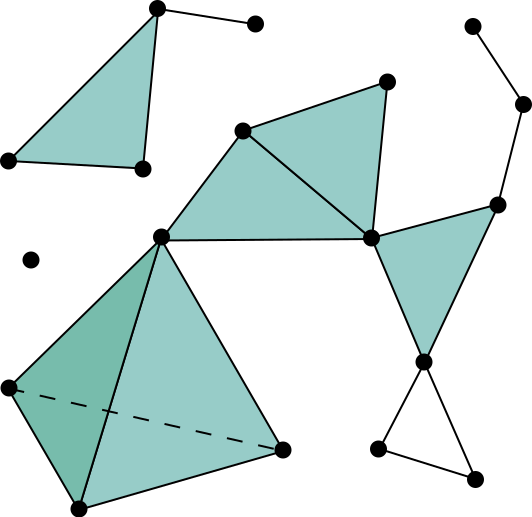
\includegraphics[width=50mm,scale=0.5]{Simplicial_complex_example.png}
    \caption{A simplicial 3-complex}
    \label{fig:fig1}
    \end{figure}
		       
 \end{frame}
 
 \begin{frame}
  Consider the following partially ordereed set  $ V = \{1, 2, 3, 4\}$: 
              The simplicial complex 
              $\mathcal{K} = \{I = \{1, 2, 3\}, \{1, 2\}, \{1, 3\}, \{2, 3\}, \{1\}, \{2\}, \{3\}, \{4\}, \emptyset\}$
             
             \begin{center}
              

              \begin{tikzpicture}[line join = round, line cap = round]

                % 0-simplex
                \coordinate [label=below:$4$] (0) at (3,1.5);
                % 2-simplex
                \coordinate [label=below:$1$] (1) at (4,0);
                \coordinate [label=below:$2$] (2) at (6,0);
                \coordinate [label=above:$3$] (3) at (5,{sqrt(3)});

                \begin{scope}[decoration={markings,mark=at position 0.5 with
                    {\arrow{to}}}]
                  % 0-simplex
                  \draw[fill] (0) circle [radius=0.03];
                  % 2-simplex
                  \draw[fill] (1) circle [radius=0.025];
                  \draw[fill] (2) circle [radius=0.025];
                  \draw[fill] (3) circle [radius=0.025];
                  \draw[thick, postaction={decorate}] (1)--(2);
                  \draw[thick, postaction={decorate}] (1)--(3);
                  \draw[thick, postaction={decorate}] (2)--(3);
                  \filldraw[opacity=.3, gray] (1) --  (2) --  (3) -- cycle;

                \end{scope}
              \end{tikzpicture}
             
             \end{center}
             
             Given an abstract simplex $\cK$, we can construct its
             \emph{topological realization}  as
             
              \[|\mathcal{K}| = \underset{\varnothing \neq I\in \cK }{\bigcup} (\textrm{Conv}(e_i),i\in I)\subseteq \RR^m\] 
              where $\{e_i\}$ is in the standard basis $e_1, \cdots e_m \in \mathbb{R}^m$.
 \end{frame}

 
  \subsection{Chain Complex}
  \begin{frame}
   \begin{definition}[Chain complex]
		      	   Complex of abelian groups.\\
		      	   A chain complex is a sequence of homomorphisms of abelian groups:
		      	   \[
                        \xymatrix{
                            {...}  \ar[r] & 
                            C_{n+1}  \ar[r]^{\partial_{n+1}} & 
                            C_n  \ar[r]^{\partial_n} & 
                            C_{n-1}  \ar[r]^{\partial_{n-1}} & 
                            {...}  \ar[r] & 
                            C_1  \ar[r]^{\partial_1} & 
                            C_0  \ar[r]^{\partial_0 = 0}
                            & 0 \\ }
                   \]
		      	   where \(\partial_n\partial_{n+1}=0\) for each n  in $\mathbb{Z}$. The equation
		      	   \(\partial_n\partial_{n+1}=0\) is equivalent to the inclusion $ \Ima\partial_{n+1} \subset \ker\partial_n $.
		      \end{definition}
            The boundary map
		      $\partial_n: \Delta_n(\mathcal{X}) \rightarrow \Delta_{n-1}(\mathcal{X})$ for the would-be chain complex $\Delta_\bullet(X)$ is defined as
		      \[
		         \partial_n(\sigma_\alpha) = \sum\limits_i (-1)^i \sigma_\alpha | [v_0, ... ,\widehat{v_i}, ... , v_n].
              \]
 \end{frame}
 
 \begin{frame}
 \frametitle{Boundary operator}
 \begin{columns}
        \begin{column}{0.4\textwidth}
            \begin{center}

                \begin{tikzpicture}[line join = round, line cap = round]
              
                                % 2-simplex
                                \coordinate [label=below:$v_0$] (3) at (4,0);
                                \coordinate [label=below:$v_1$] (4) at (6,0);
                                \coordinate [label=above:$v_2$] (5) at (5,{sqrt(3)});
                                \coordinate (0) at (4.8, 0.5);
                               
                                
                                \begin{scope}[decoration={markings,mark=at position 0.5 with {\arrow{to}}}]
                                    
                                  
                                    \draw[fill] (3) circle [radius=0.025];
                                    \draw[fill] (4) circle [radius=0.025];
                                    \draw[fill] (5) circle [radius=0.025];
                                    \draw[thick, postaction={decorate}] (3)--(4) node [midway, below] {a};
                                    \draw[thick, postaction={decorate}] (3)--(5) node [near start, above=10pt] {c};

                                    \draw[thick, postaction={decorate}] (4)--(5) node [near start, above=10pt] {b};
                                    \draw[->,>=latex'] (0) arc[radius=0.25,start angle=225,delta angle=300];
                                    
                                \end{scope}
                \end{tikzpicture} 
            \end{center}
        \end{column}
\begin{column}{0.6\textwidth}  %%<--- here
     $\partial[v_0, v_1] = v_1 - v_0$ \\~\\
     $\partial[v_0, v_1, v_2] = [v_0, v_1] + [v_1, v_2] - [v_0, v_2]$ \\ 
    
\end{column}
\end{columns}
  
 \end{frame}

 \begin{frame}
  \frametitle{Homology of a Chain Complex}
        \begin{definition}[Homology Group]
            The n-th homology group of the chain complex is defined as the quotient group
            \[ 
            H_n = \frac{Z_n}{B_n} = \frac{\ker\partial_n}{\Ima\partial_{n+1}}
            \]
            Elements of $Z_n$ are called cycles and elements of $B_n$ are called boundaries.
  \end{definition}
      Elements of $H_n$ are cosets of $\Ima\partial_{n+1}$,
      called homology classes. Two cycles representing the same homology class are said
      to be homologous. This means their difference is a boundary.
 \end{frame}

  \subsection{Computing Homology}

 \begin{frame}
 \frametitle{Computing Homology of $\mathbb{R} \mathbb{P}^2$ in $\mathbb{Z}$}
 
 One way to calculate the homology groups of a projective plain $\mathbb{R} \mathbb{P}^2$ is by triangulating it into two 2-simplices A and B, upper triangle and lower one respectively.

	\[
		\xymatrix{
			w \ar @{} [d]^(0.3) {\;\, A }
			& v  \ar[l]_b \ar[d]^a  \\
			v \ar[u]^a \ar[r]_b \ar[ur]|{c}
			& w \ar @{} [u]^(0.3) {B \;\, } }
	\]
	
	We can construct the following chain complex which is a sequence of homomorphisms of abelian groups:

    \[
		\xymatrix{
			0  \ar[r]^{\partial_3 = 0} &
			C_2  \ar[r]^{\partial_2} &
			C_1  \ar[r]^{\partial_1} &
			C_0  \ar[r]^{\partial_0 = 0}
			& 0 \\ }
	\]

 where \(\partial_n\partial_{n+1}=0\) for each n  in $\mathbb{Z}$
 \end{frame}
 
 \begin{frame}
  \[
				\left|
				  \begin{array}{l}
				  	C_0=\langle v,w \rangle\\
				  	C_1=\langle a, b, c \rangle\\
                                C_2=\langle A, B \rangle\\
				      C_n=\{0\} \quad \forall n \geqslant 3
				  \end{array}
				\right.,
			\]

    \[
		\xymatrix{
			0  \ar[r]^{\partial_3 = 0} &
			\mathbb{Z}^{\oplus^2}  \ar[r]^{\partial_2} &
			\mathbb{Z}^{\oplus^3}  \ar[r]^{\partial_1} &
			\mathbb{Z}^{\oplus^2}  \ar[r]^{\partial_0 = 0}
			& 0 \\ }
	\]
The n-th homology group is defined as $H_n= \ker\partial_n\left/ \Ima \partial_n \right.$
\\
The homology groups of the projective plane are:
		\[
	  		H_n^\Delta(\mathbb{R} \mathbb{P}^2) \simeq \left\{
			      \begin{array}{rl}
			     \mathbb{Z}, & \textrm{for} \: n = 0\\
			     \frac{\mathbb{Z}}{2\mathbb{Z}}, & \textrm{for} \: n = 1\\
                        0 & \textrm{for} \: n \geqslant 2
			      \end{array}
			 \right.
	  	\]

\end{frame}

\begin{frame}
Let's compute $H_1$: \\
$\ker\partial_1 = \langle a-b,c \rangle$
		since $\partial_1(\alpha a + \beta b + \gamma c) = (\alpha + \beta)(w-v) = 0  \implies \alpha = -\beta$ \\
The general element in $C_1$: $ (\alpha a + \beta b + \gamma c)= \alpha(a-b) + \gamma c $,
so the $\ker\partial_1$ can be generated by the elements a-b and c \\
$\Ima\partial_2 = \langle -a+b+c,\, a-b+c \rangle $
		since $\partial_2(\alpha A + \beta B) = \alpha(-a+b+c) + \beta(a-b+c)$ \\
$H_1 = \frac{\ker\partial_1}{\Ima\partial_2} =
		\frac{ \langle a-b, \,c \rangle  }{ \langle -a+b+c,\, a-b+c \rangle }$\\
The group $\langle a-b, c \rangle$ can be also generated by the elements
		$ m=a-b+c, and \: c $ where $ a - b = m -c $. So, \\
$H_1 = \frac{ \langle a-b, \,c \rangle  }{ \langle -a+b+c,\, a-b+c \rangle } = \frac{ \langle a-b+c, \, c \rangle  }{ \langle a-b+c,\, -a+b+c \rangle } $ \\
If we let $t=a-b+c$ then $-a+b+c = -t + 2c $ then the group $\langle t,\, -t+2c \rangle$ can be also generated by the elements $ t \: and \: 2c $. \\
In terms of t and c, $H_1 = \frac{ \langle t, \,c \rangle  }{ \langle t,\, 2c \rangle } = \frac{  \langle c \rangle  }{ \langle 2c \rangle } \simeq \frac{\mathbb{Z}}{2\mathbb{Z}}$
 \end{frame}

 \begin{frame}
 \frametitle{Maps of Chain Complexes}

     Let $(C_\bullet, \partial)$ and $(D_\bullet, \delta)$ be two chain complexes.
     A map of chain complexes is a morphism $f$ that is a sequence of homomorphisms $(f_n)_{n  \in  Z}$:

            \[
                  \begin{tikzcd}[ampersand replacement=\&]
                    (C_\bullet, \partial) \& C_\bullet \ \ldots \arrow[r]  \& C_n \arrow[r, "\partial n"] \arrow[d, "{f_n}"]   \& C_{n-1} \arrow[r, "\partial {n-1}"] \arrow[d, "f_{n-1}"]   \& C_{n-2} \arrow[r, "\partial {n-2}"] \arrow[d, "f_{n-2}"]    \& \ldots \ C_\bullet \\
                    (D_\bullet, \delta) \& D_\bullet \ \ldots \arrow[r]    \& D_n \arrow[r, "\delta n"]    \& D_{n-1} \arrow[r, "\delta {n-1}"]    \& D_{n-2} \arrow[r, "\delta {n-2}"]   \& \ldots \ D_\bullet \\
                  \end{tikzcd}
                \]
            \[
                  f_n : C_n \rightarrow D_n \quad s.t, \quad   f_{n-1} \circ \partial n = \delta_n \circ f_n \; \forall n \in \mathbb{Z}
                  \]
                   \[
                  \begin{tikzcd}[ampersand replacement=\&]
                    \& C_n \arrow[r, "\partial n"] \arrow[d, "{f_n}"]    \& C_{n-1} \arrow[d, "{f_{n-1}}"] \\
                    \& D_n \arrow[r, "\delta n"]    \& D_{n-1} \\
                  \end{tikzcd}
                   \quad         commutes.
                \]
 \end{frame}

 \begin{frame}
 \frametitle{Maps of Chain Complexes induce Maps on Homology}
   A homomorphism of chain complexes induces a homomorphism on the homology.
                The induced map can be defined as:
               \begin{align*}
                  H_n(f) &:  H_n(C_\bullet) \rightarrow H_n(D_\bullet)  \\
                  H_n(f) &: [x] \mapsto [f_n(x)]
                \end{align*}

                To prove the claim above it is enough to check that $H_n(f)$ is well-defined.
                We can prove well-defines by checking if cycles are send to cycles and boundaries to boundaries. \\

                (1) Let us take a cycle $x \in C_n$, so that $x \in \ker (\partial_n)$, $\partial_n(x) = 0$

                    \begin{align*}
                        \delta_n \circ f_n(x) = f_{n-1} \circ \partial n(x) = f_{n-1}(0) = 0
                        &\Rightarrow f_n(x) \in \ker \delta_n , f_n(x) \, is \, a \, cycle \\
                        &\Rightarrow f_n(\ker \partial n) \subseteq \ker \delta_n \\
                    \end{align*}
                      So, cycles are send to cycles.

 \end{frame}

 \begin{frame}
                (2) Let us take a boundary $y \in C_n$, so that $y \in \Ima\partial_{n+1}$
                $\Rightarrow \exists z \in C_{n+1}$ such that $\partial_{n+1}(z) = y$
                \begin{align*}
                  &\null f_n(y) = f_n(\partial_{n+1}(z))  = \delta_{n+1}(f_{n+1}(z)) \\
                  &\null \Rightarrow f_n(y) \in \Ima\partial_{n+1} f_n(y) \, is \, a \, boundary\\
                  &\null \Rightarrow f_n(Im\partial_{n+1}) \subseteq Im(\delta_{n+1})
                \end{align*}
                So, boundaries are send to boundaries.

                \begin{align*}
                   H_n(f) &:  H_n(C_\bullet) \rightarrow H_n(D_\bullet)  \\
                   H_n(f) &:  \ker{\partial_n} \left/ \Ima(\partial_{n+1}) \right. \rightarrow \ker{\delta_n} \left/ \Ima(\delta_{n+1}) \right. \\
                             & [x] \mapsto [f_n(x)] \\
                             & x + \Ima\partial_{n+1} \mapsto f_n(x) + f_n(\Ima\delta_{n+1}) =  f_n(x) + Im(\delta_{n+1}) = [f_n(x)]
                \end{align*}
 \end{frame}

 
%  \begin{frame}
%   \frametitle{Computing Homology of $S^1$ in $\mathbb{Z}$}
% 
% Space $\mathcal{X} = S^1$  \\~\\
%         \begin{figure}
%             \begin{tikzpicture}[line join = round, line cap = round]
%               
%                                 2-simplex
%                                 \coordinate [label=below:$v_0$] (3) at (3,0);
%                                 \coordinate [label=below:$v_1$] (4) at (5,0);
%                                 \coordinate [label=above:$v_2$] (5) at (4,{sqrt(3)});
%                                 \coordinate [label=above:$\simeq$] (1) at (2,0.5);
%                                 \coordinate (0) at (3.8, 0.5);
%                                 
%                                 \begin{scope}[decoration={markings,mark=at position 0.5 with {\arrow{to}}}]
%                                     
%                                     \draw[fill] (1) circle [radius=0];
%                                     \draw[fill] (3) circle [radius=0.025];
%                                     \draw[fill] (4) circle [radius=0.025];
%                                     \draw[fill] (5) circle [radius=0.025];
%                                     
%                                     \draw[thick, postaction={decorate}] (3)--(4) node [midway, below] {a};
%                                     \draw[thick, postaction={decorate}] (3)--(5) node [near start, above=10pt] {c};
%                                     \draw[thick, postaction={decorate}] (4)--(5) node [near start, above=10pt] {b};
%                                     \draw[->,>=latex'] (0) arc[radius=0.25,start angle=225,delta angle=300];
%                                     \draw[thick] (0,{sqrt(3)/2}) circle (1.2cm);
% 
%                                     
%                             \end{scope}
%                 \end{tikzpicture} 
%                 \caption{Triangulation of $S^1$}
%             \end{figure}
%             
%  \end{frame}
%  
%  \begin{frame}
%  
%    We can construct the following chain complex which is a sequence of homomorphisms of abelian groups: 
% 
% 	\[
% 		\xymatrix{
% 			0  \ar[r]^{\partial_2 = 0} & 
% 			C_1  \ar[r]^{\partial_1} & 
% 			C_0  \ar[r]^{\partial_0 = 0}
% 			& 0 \\ }
% 	\]
% 
%  where \(\partial_n\partial_{n+1}=0\) for each n  in $\mathbb{Z}$ and 
%  
% 			\[
% 				\left|
% 				  \begin{array}{l}
% 				  	C_0= \langle v_0, v_1, v_2 \rangle \\
% 				  	C_1=\langle a, b, c \rangle \\
%                     C_n=\{0\} \quad \forall n \geqslant 2 
% 				  \end{array}
% 				\right., 
% 			\]
% 
% 			\[
%                 \xymatrix{
%                     0  \ar[r]^{\partial_2 = 0} & 
%                     \mathbb{Z}^{\oplus^3}  \ar[r]^{\partial_1} & 
%                     \mathbb{Z}^{\oplus^3}  \ar[r]^{\partial_0 = 0}
%                     & 0 \\ }
% 	        \]
% 	        
%  \end{frame}
%  
%     \begin{frame}
%     \frametitle{$H_0$ - \# of connected components}
%             The n-th homology group is defined as $H_n = \frac{\ker\partial_n}{\Ima\partial_{n+1}}$. \\
% 
% 
% First, let's compute $H_0$: 
% 
% $\ker\partial_0 = C_0 = \langle v_0, v_1, v_2 \rangle$ since $\partial_0 = 0$.
% 
% To calculate $\Ima\partial_1$, let's compute:
% $\partial_1(\alpha a + \beta b + \gamma c) = \alpha (v_1-v_0) + \beta (v_2-v_1) - \gamma (v_2-v_0) 
% = (\gamma -\alpha)v_0 + (\alpha - \beta)v_1 + (-(\gamma - \alpha)-(\alpha - \beta))v_2 $ 
%  \[ \Ima\partial_1 = \left\{ \left(\begin{array}{c}
%           		                 	( \gamma - \alpha )\\
%           		                 	(\alpha - \beta)\\
%           		                 	-(\gamma - \alpha)-(\alpha - \beta)\\
%           		                 \end{array} \right), \quad \alpha, \beta, \gamma \subseteq \mathbb{Z} \right\} 
%           		                 \subseteq \mathbb{Z}^{\oplus^3} \]
%     There exist an isomorphism $\Ima\partial_1 \simeq \mathbb{Z}^2$
%     
% $H_0 = \frac{\ker\partial_0}{\Ima\partial_1} = \mathbb{Z}^{3} \left/ {
%     \left(\begin{array}{c}
%                     1\\
%                     0\\
%                     -1\\
%             \end{array} \right)\mathbb{Z} \oplus
%     \left(\begin{array}{c}
%                     0\\
%                     1\\
%                     -1\\
%             \end{array} \right)\mathbb{Z}} \right. \simeq \mathbb{Z}$ 
% 
%     \end{frame}
%  
%   \begin{frame}
%   \frametitle{$H_1$ - \# of holes}
%         Second, let's compute $H_1$: \\
%         $\ker\partial_1 = \left\{ \left(\begin{array}{c}
%                             m\\
%                             m\\
%                             m\\
%                     \end{array} \right), m \in \mathbb{Z} = \right\} = \left(\begin{array}{c}
%                             1\\
%                             1\\
%                             1\\
%                     \end{array} \right) \mathbb{Z} \simeq \mathbb{Z}$ \\ 
%         $\Ima\partial_2 = \{0\}$ since $C_2 = \{0\}$ \\
%         $H_1 = \frac{\ker\partial_1}{\Ima\partial_2} = 
%                 \frac{ \ker{\partial_1} }{ \{0\} } = \ker{\partial_1} \simeq \mathbb{Z}$ 
% 
%                 
%         Finally, the homology groups of the circle are: 
%                 \[
%                     H_n^\Delta(S^1) \simeq \left\{
%                         \begin{array}{rl}
%                         \mathbb{Z}, & \textrm{for} \: n = 0, 1\\
%                         
%                                 0 & \textrm{for} \: n \geqslant 2
%                         \end{array}
%                     \right.
%                 \]
%  \end{frame}


  \section{Maps of Complexes and Maps on Homology}
  
  \begin{frame}
  \frametitle{Filtered Complex}
  \begin{figure}
                    $\mathcal{X}$  \hspace{3.5cm}  $\mathcal{Y}$  \hspace{3.5cm}  $\mathcal{Z}$ \\~\\
                    
                    
  \begin{tikzpicture}[line join = round, line cap = round]

                        % first-simplex
                        \coordinate [label=below:$v_0$] (0) at (0,0);
                        \coordinate [label=below:$v_1$] (1) at (2,0);
                        \coordinate [label=above:$v_2$] (2) at (1,{sqrt(3)});
                       
                         % second-simplex
                        \coordinate [label=below:$v_0$] (3) at (4,0);
                        \coordinate [label=below:$v_1$] (4) at (6,0);
                        \coordinate [label=above:$v_2$] (5) at (5,{sqrt(3)});
                        
                        % third-simpex
                        \coordinate [label=below:$v_0$] (6) at (8,0);
                        \coordinate [label=below:$v_1$] (7) at (10,0);
                        \coordinate [label=above:$v_2$] (8) at (9,{sqrt(3)});

                        \begin{scope}[decoration={markings,mark=at position 0.5 with
                            {\arrow{to}}}]
                            % first-simplex
                            \draw[fill] (0) circle [radius=0.03];
                            \draw[fill] (1) circle [radius=0.03];
                            \draw[fill] (2) circle [radius=0.03];
                            \draw [thin, right hook->] (2.75, 0.86) -- (3.25, 0.86);  
                            % second-simplex
                            \draw[fill] (3) circle [radius=0.03];
                            \draw[fill] (4) circle [radius=0.03];
                            \draw[fill] (5) circle [radius=0.03];
                            \draw[thick, postaction={decorate}] (3)--(4);
                            \draw[thick, postaction={decorate}] (3)--(5);
                            \draw[thick, postaction={decorate}] (4)--(5);
                           \draw [thin, right hook->] (6.75, 0.86) -- (7.25, 0.86);  
                           % third-simpex
                            \draw[fill] (6) circle [radius=0.03];
                            \draw[fill] (7) circle [radius=0.03];
                            \draw[fill] (8) circle [radius=0.03];
                            \draw[thick, postaction={decorate}] (6)--(7);
                            \draw[thick, postaction={decorate}] (6)--(8);
                            \draw[thick, postaction={decorate}] (7)--(8);
                            \filldraw[opacity=.3, gray] (6) --  (7) --  (8) -- cycle;
                        \end{scope}

                    \end{tikzpicture} 
                    
                    
                    
                     $C_\bullet^0  \longrightarrow   C_\bullet^1   \longrightarrow C_\bullet^2$  \\~\\
                    
                    
                    \end{figure}
 \end{frame}
 
 \begin{frame}
 \frametitle{Maps of Complexes}
 \footnotesize
 \setlength{\arraycolsep}{0.5pt}
 \medmuskip = 0mu % default: 4mu plus 2mu minus 4mu
 \[
                    \begin{tikzcd}[ampersand replacement=\&]
  \& C_\bullet^0   \arrow[rr]                                     \&  \& C_\bullet^1 \arrow[rr]                               \&  \& C_\bullet^2                                                                 \\ \\
  \& 0 \arrow[d]                                         \&  \& 0 \arrow[d]                                         \&  \& 0 \arrow[d]                                                                 \\ 
2 \& 0 \arrow[rr] \arrow[d, "\partial^0_2=0"]            \&  \& 0 \arrow[rr] \arrow[d, "\partial^1_2=0"]            \&  \& \mathbb{Z} \arrow[d, "\partial_2^2 = {\begin{pmatrix} 1 \\ 1  \\  -1  \end{pmatrix}}"] \\
1 \& 0 \arrow[d, "\partial^0_1=0"] \arrow[rr]            \&  \& \mathbb{Z}^3 \arrow[rr] \arrow[d, "\partial_1^1 = \partial_1^2"]                   \&  \& \mathbb{Z}^3 \arrow[d, "\partial_1^2 = {\begin{pmatrix} -1 & 0 & -1 \\ 1 & -1 & 0 \\ 0 & 1 & 1 \end{pmatrix}}"]                                                      \\
0 \& \mathbb{Z}^3 \arrow[d, "\partial^0_0=0"] \arrow[rr] \&  \& \mathbb{Z}^3 \arrow[rr] \arrow[d, "\partial^1_0=0"] \&  \& \mathbb{Z}^3 \arrow[d, "\partial^2_0=0"]                                    \\
  \& 0                                                   \&  \& 0                                                   \&  \& 0                                                                          
\end{tikzcd}
\]
    \end{frame}

    
 \begin{frame}
 \frametitle{Maps of Complexes induce maps on Homology}
 \footnotesize
 \setlength{\arraycolsep}{0.5pt}
 \medmuskip = 0mu % default: 4mu plus 2mu minus 4mu
 \[
                    \begin{tikzcd}[ampersand replacement=\&]
  \& H(C_\bullet^0)   \arrow[rr]                                     \&  \& H(C_\bullet^1) \arrow[rr]                               \&  \& H(C_\bullet^2)                                                                 \\ \\
  \& 0 \arrow[d]                                         \&  \& 0 \arrow[d]                                         \&  \& 0 \arrow[d]                                                                 \\ 
2 \& 0 \arrow[rr] \arrow[d]            \&  \& 0 \arrow[rr] \arrow[d]            \&  \& 0 \arrow[d] \\
1 \& 0 \arrow[d] \arrow[rr]            \&  \& \mathbb{Z} \arrow[rr] \arrow[d]                   \&  \& 0 \arrow[d]                                              \\
0 \& \mathbb{Z}^3 \arrow[d] \arrow[rr] \&  \& \mathbb{Z} \arrow[rr] \arrow[d] \&  \& \mathbb{Z} \arrow[d]                                    \\
  \& 0                                                   \&  \& 0                                                   \&  \& 0                                                                          
\end{tikzcd}
\]
    \end{frame}
    
    
    \begin{frame}
     Consider a short exact sequence of chain complexes: \\
                \[
                0 \rightarrow A_\bullet \xrightarrow{i} B_\bullet \xrightarrow{\pi} C_\bullet \rightarrow 0
                \]

                $A_\bullet, \ B_\bullet, \ C_\bullet$ are chain complexes and $i, \pi$ are maps between chain complexes where
                $\ker \pi = \Ima i, \quad \pi:surjective \ and \ i: injective$\\
                induces long exact sequence of homology:\\
                \begin{align*}
                H_{n+1}(C_\bullet) \xrightarrow{\partial n+1} H_n(A_\bullet) \xrightarrow{i_*} H_n(B_\bullet) \xrightarrow{\pi_*} H_n(C_\bullet) \xrightarrow{\delta} H_{n-1}(A_\bullet) \rightarrow \\ H_{n-1}(B_\bullet) \rightarrow H_{n-1}(C_\bullet) \\
                \end{align*}
    \end{frame}

    \begin{frame}
     \frametitle{The Equivalence of Simplicial and Singular Homology}
     singular $n-simplex$ in a space $X$ is a map $\sigma: \Delta^n \rightarrow X$
     We considered a parameterization of a space by simplexes, where the maps $\sigma_\alpha: \Delta^n \rightarrow X$ had restrictions. If we only require that the $\sigma$ map is continous, then by definition that would be a singular $n-simplex$ in a space $X$.\\
     The lack of other restrictions on the map $\sigma: \Delta^n \rightarrow X$, convey that $\sigma$ does not need to be a `nice` embedding, in fact it can have singularities, where its image does not look like a simplex.

     $C_n(X)$ is a free abelian group with generators the set of singluar $n-simplexes$ in X: the continous maps $\sigma: \Delta^n \rightarrow X$.
     \begin{theorem}
     The homomorphisms $H^{\Delta}_{n}(X,A) \rightarrow H_n(X,A)$ are isomorphisms for
all $n$ and all $\Delta$-complex pairs $(X, A)$.
     \end{theorem}
    \end{frame}

    \begin{frame}
     In addition to the long exact sequence of homology groups for a pair $(X, A)$, there is another sort of long exact sequence, known as a Mayer-Vietoris sequence, which is equally powerful but is sometimes more convenient to use. For a pair of subspaces $A, B \subset X$ such that $X$ is the union of the interiors of $A$ and $B$ , this exact sequence has the form
     \[ ... \rightarrow H_n(A \cap B) \xrightarrow{\phi} H_n(A) \oplus H_n(B) \xrightarrow{\Psi} H_n(X) \xrightarrow{\partial} H_{n-1}(A \cap B) \rightarrow ... \rightarrow H_0(X) \rightarrow 0 \]
     \\
      The Mayer-Vietoris sequence is then the long exact sequence of homology groups associated to the short exact sequence of chain complexes formed by the short exact sequences
      \[ 0 \rightarrow C_n(A \cap B) \xrightarrow{\Phi} C_n(A) \oplus C_n(B) \xrightarrow{\Psi} C_n(A + B) \rightarrow 0 \]
    \end{frame}
    
    \begin{frame}
    \frametitle{The Nerve Theorem}
      If $X$ is a topological space, and $X = \underset{\alpha}{\cup} \quad \mathcal{U}_\alpha$ 
             where $\mathcal{U} = \{\mathcal{U}_\alpha\}_{\alpha\in A}$ are cover indexes, $\mathcal{U} = \{\mathcal{U}_1, \mathcal{U}_2, \cdots, \mathcal{U}_n\}$, given a cover $\mathcal{U}$ (not necessarily open) of a space $X$, the nerve of $\mathcal{U}$ is a simplicial complex  $\mathcal{N}(\mathcal{U})$ whose n-simplices consist of sets of $n+1$ elements of $\mathcal{U}$ with non-empty intersections.
              Vertices of $\mathcal{N}(\mathcal{U})= \{1, 2, \cdots, m\}$ are 
              $(k - 1)$ - faces if $\ \mathcal{U}_{i_{1}} \cap \cdots \cap \mathcal{U}_{i_{k}} 
              \ne \emptyset$ for $ \{i_1, \cdots, i_k \} \in \mathcal{N}(\mathcal{U})$
              \\
              \begin{theorem}[The Nerve Theorem]
              
            If $X$ is a paracompact space, and $U$ is an open cover of $X$ such that the
            intersection of any finite subfamily of $U$ is either empty or contractible,
            then the realization of the nerve of $U$ is homotopy equivalent to X.
            
              \end{theorem}
    \end{frame}


    
    \section{\v{C}ech and Vietoris-Rips Complex}
    \subsection{Definition}
 \begin{frame}
If $\mathcal{X}$ is a metric space and $r \geq 0$:
\begin{definition} [\v{C}ech Complex]
           Given a collection of points $\{x_\alpha\}$ in Euclidean space $\mathbb{E}^n$, the \v{C}ech Complex, $\mathcal{C}_\epsilon$, is the abstract simplicial complex whose k-simplices are determined by unordered (k+1)-uple of points $\{x_\alpha\}_0^k$ whose closed $\epsilon/2-ball$ neighborhoods have a point of common intersection. 
 \end{definition}
 \begin{definition} [Vietoris-Rips Complex]
              Given a collection of points $\{x_\alpha\}$ in Euclidean space $\mathbb{E}^n$, the Rips Complex, $\mathcal{R}_\epsilon$, is the abstract simplicial complex whose k-simplices correspond to unordered (k+1)-uple of points $\{x_\alpha\}_0^k$ which are pairwise within distance $\epsilon$.
 \end{definition}
 
 Relation of \v{C}ech and Vietoris-Rips Complex: 
 For each $\epsilon > 0$, there is a chain inclusion maps
    \[
     \mathcal{R} \hookrightarrow \mathcal{C}_{\epsilon\sqrt{2}} \hookrightarrow \mathcal{R}_{\epsilon\sqrt{2}}
    \]

 
 \end{frame}


  \subsection{\v{C}ech Complex Example}
  \begin{frame}
  \frametitle{\v{C}ech Complex Example}
  \begin{tikzpicture}[line join = round, line cap = round]

                        % first-simplex
                        \coordinate (0) at (0,0);
                        \coordinate (1) at (2,0);
                        \coordinate (2) at (1,{sqrt(3)});
                       
                         % second-simplex
                        \coordinate  (3) at (4,0);
                        \coordinate  (4) at (6,0);
                        \coordinate  (5) at (5,{sqrt(3)});
                        
                        % third-simpex
                        \coordinate  (6) at (8.5,0);
                        \coordinate  (7) at (10.5,0);
                        \coordinate  (8) at (9.5,{sqrt(3)});

                        \begin{scope}[decoration={markings,mark=at position 0.5 with
                            {\arrow{to}}}]
                            
                            % first-simplex
                            \draw[fill] (0) circle [radius=0.05];
                            \draw[fill, opacity=0.3, blue] (0) circle [radius=0.3];
                            \draw[fill] (1) circle [radius=0.05];
                            \draw[fill, opacity=0.3, blue] (1) circle [radius=0.3];
                            \draw[fill] (2) circle [radius=0.05];
                            \draw[fill, opacity=0.3, blue] (2) circle [radius=0.3];
                            \draw [thin, right hook->] (2.75, 0.86) -- (3.25, 0.86);  
                            
                            % second-simplex
                            \draw[fill] (3) circle [radius=0.05];
                            \draw[fill, opacity=0.3, blue] (3) circle [radius=1.05];
                            \draw[fill] (4) circle [radius=0.05];
                            \draw[fill, opacity=0.3, blue] (4) circle [radius=1.05];
                            \draw[fill] (5) circle [radius=0.05];
                            \draw[fill, opacity=0.3, blue] (5) circle [radius=1.05];
                            \draw[thick] (3)--(4);
                            \draw[thick] (3)--(5);
                            \draw[thick] (4)--(5);
                            \draw [thin, right hook->] (6.75, 0.86) -- (7.25, 0.86);  
                            
                           % third-simpex
                            \draw[fill] (6) circle [radius=0.05];
                            \draw[fill, opacity=0.3, blue] (6) circle [radius=1.2];
                            \draw[fill] (7) circle [radius=0.05];
                            \draw[fill, opacity=0.3, blue] (7) circle [radius=1.2];
                            \draw[fill] (8) circle [radius=0.05];
                            \draw[fill, opacity=0.3, blue] (8) circle [radius=1.2];
                            \draw[thick] (6)--(7);
                            \draw[thick] (6)--(8);
                            \draw[thick] (7)--(8);
                            \filldraw[opacity=.5, gray] (6) --  (7) --  (8) -- cycle;
                        \end{scope}

                    \end{tikzpicture} 
                    
 \end{frame}
 
 \subsection{Vietoris-Rips Complex Example}
 \begin{frame}
  \frametitle{Vietoris-Rips Complex Example}
  \begin{tikzpicture}[line join = round, line cap = round]

                       % first-simplex
                        \coordinate (0) at (0,0);
                        \coordinate (1) at (2,0);
                        \coordinate (2) at (1,{sqrt(3)});
                       
                         % second-simplex
                        \coordinate  (3) at (4,0);
                        \coordinate  (4) at (6,0);
                        \coordinate  (5) at (5,{sqrt(3)});
                        
                        % third-simpex
                        \coordinate  (6) at (8.5,0);
                        \coordinate  (7) at (10.5,0);
                        \coordinate  (8) at (9.5,{sqrt(3)});

                        \begin{scope}[decoration={markings,mark=at position 0.5 with
                            {\arrow{to}}}]
                            % first-simplex
                            \draw[fill] (0) circle [radius=0.05];
                            \draw[fill, opacity=0.3, blue] (0) circle [radius=0.3];
                            \draw[fill] (1) circle [radius=0.05];
                            \draw[fill, opacity=0.3, blue] (1) circle [radius=0.3];
                            \draw[fill] (2) circle [radius=0.05];
                            \draw[fill, opacity=0.3, blue] (2) circle [radius=0.3];
                            \draw [thin, right hook->] (2.75, 0.86) -- (3.25, 0.86);  
                            % second-simplex
                            \draw[fill] (3) circle [radius=0.05];
                            \draw[fill, opacity=0.3, blue] (3) circle [radius=1.05];
                            \draw[fill] (4) circle [radius=0.05];
                            \draw[fill, opacity=0.3, blue] (4) circle [radius=1.05];
                            \draw[fill] (5) circle [radius=0.05];
                            \draw[fill, opacity=0.3, blue] (5) circle [radius=1.05];

                            \draw[thick] (3)--(4);
                            \draw[thick] (3)--(5);
                            \draw[thick] (4)--(5);
                           \draw [thin, right hook->] (6.75, 0.86) -- (7.25, 0.86);  
                            \filldraw[opacity=.5, gray] (3) --  (4) --  (5) -- cycle;
                           % third-simpex
                            \draw[fill] (6) circle [radius=0.05];
                            \draw[fill, opacity=0.3, blue] (6) circle [radius=1.2];
                            \draw[fill] (7) circle [radius=0.05];
                            \draw[fill, opacity=0.3, blue] (7) circle [radius=1.2];
                            \draw[fill] (8) circle [radius=0.05];
                            \draw[fill, opacity=0.3, blue] (8) circle [radius=1.2];
                            \draw[thick] (6)--(7);
                            \draw[thick] (6)--(8);
                            \draw[thick] (7)--(8);
                            \filldraw[opacity=.5, gray] (6) --  (7) --  (8) -- cycle;
                        \end{scope}

                    \end{tikzpicture} 
                    
 \end{frame}
 \begin{frame}
\begin{figure}
    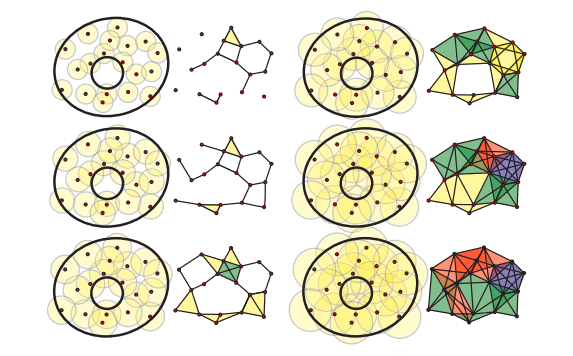
\includegraphics[width=80mm,scale=1.5]{rips_of_annulus.png}
    \caption{A sequence of Rips Complex from a point clound data set that represent an annulus}
    \label{fig:fig1}
    \end{figure}

            \end{frame}
    
\section{Persistent Homology}

\subsection{Persistance}

\begin{frame}
\begin{definition}
 
    Given a filtered complex, the i-th complex $K^{i}$ has associated boundary operators 
    $\partial^{i_{k}}$, matrices $M^i_k$ , and groups $C^i_k$, $Z^i_k$, $B^i_k$, and $H^i_k$ for all $i, k \geq 0$
    The p-persistent k-th homology group of $K^i$ is 
            \[
             H_k^{i, p} = Z_k^i \left/ (B_k^{i+p} \cap Z_k^i) \right.
            \]

\end{definition}
             \vspace{0.5in}
             Example: 
             p = i = k = 1: $ H_1^{1, 1} = Z_1^1 \left/ (B_2^{1} \cap Z_1^1) \right. \mathbb{Z} \left/ ( \{0\} \cap \mathbb{Z}) \right. = \mathbb{Z}$

\end{frame}

\begin{frame}
  \begin{tikzpicture}[line join = round, line cap = round]
                % 1st
                \coordinate [label=above:$a$] (0) at (0,1);
                \coordinate [label=above:$b$] (1) at (1,1);
                % arrow 1st to 2nd
                \coordinate (a1) at (1.3, 0.5);
                \coordinate (a2) at (1.7, 0.5);
                % 2nd
                \coordinate [label=above:$a$] (2) at (2,1);
                \coordinate [label=below:$d$] (3) at (2,0);
                \coordinate [label=above:$b$] (4) at (3,1);
                \coordinate [label=below:$c$] (5) at (3,0);
                % arrow 2nd to 3rd
                \coordinate (a3) at (3.3, 0.5);
                \coordinate (a4) at (3.7, 0.5);
                % 3rd
                \coordinate [label=above:$a$] (6) at (4,1);
                \coordinate [label=below:$d$] (7) at (4,0);
                \coordinate [label=above:$b$] (8) at (5,1);
                \coordinate [label=below:$c$] (9) at (5,0);
                % arrow 3rd to 4th
                \coordinate (a5) at (5.3, 0.5);
                \coordinate (a6) at (5.7, 0.5);
                % 4th
                \coordinate [label=above:$a$] (10) at (6,1);
                \coordinate [label=below:$d$] (11) at (6,0);
                \coordinate [label=above:$b$] (12) at (7,1);
                \coordinate [label=below:$c$] (13) at (7,0);
                % arrow 4th to 5th
                \coordinate (a7) at (7.3, 0.5);
                \coordinate (a8) at (7.7, 0.5);
                % 5th
                \coordinate [label=above:$a$] (14) at (8,1);
                \coordinate [label=below:$d$] (15) at (8,0);
                \coordinate [label=above:$b$] (16) at (9,1);
                \coordinate [label=below:$c$] (17) at (9,0);
                % arrow 5th to 6th
                \coordinate (a9) at (9.3, 0.5);
                \coordinate (a10) at (9.7, 0.5);
                % 6th
                \coordinate [label=above:$a$] (18) at (10,1);
                \coordinate [label=below:$d$] (19) at (10,0);
                \coordinate [label=above:$b$] (20) at (11,1);
                \coordinate [label=below:$c$] (21) at (11,0);

                \begin{scope}[decoration={markings,mark=at position 0.5 with {\arrow{to}}}]
                  \draw[fill] (0) circle [radius=0.03];
                  \draw[fill] (1) circle [radius=0.03];
                  \draw[fill] (2) circle [radius=0.03];
                  \draw[fill] (3) circle [radius=0.03];
                  \draw[fill] (4) circle [radius=0.03];
                  \draw[fill] (5) circle [radius=0.03];
                  \draw[fill] (6) circle [radius=0.03];
                  \draw[fill] (7) circle [radius=0.03];
                  \draw[fill] (8) circle [radius=0.03];
                  \draw[fill] (9) circle [radius=0.03];
                  \draw[fill] (10) circle [radius=0.03];
                  \draw[fill] (11) circle [radius=0.03];
                  \draw[fill] (12) circle [radius=0.03];
                  \draw[fill] (13) circle [radius=0.03];
                  \draw[fill] (14) circle [radius=0.03];
                  \draw[fill] (15) circle [radius=0.03];
                  \draw[fill] (16) circle [radius=0.03];
                  \draw[fill] (17) circle [radius=0.03];
                  \draw[fill] (18) circle [radius=0.03];
                  \draw[fill] (19) circle [radius=0.03];
                  \draw[fill] (20) circle [radius=0.03];
                  \draw[fill] (21) circle [radius=0.03];
                  % hooks
                  \draw [right hook->] (a1) -- (a2);
                  \draw [right hook->] (a3) -- (a4);
                  \draw [right hook->] (a5) -- (a6);
                  \draw [right hook->] (a7) -- (a8);
                  \draw [right hook->] (a9) -- (a10);
                  % 2nd
                  \draw[thick] (5)--(4);
                  \draw[thick] (2)--(4);
                  % 3rd
                  \draw[thick] (6)--(7);
                  \draw[thick] (6)--(8);
                  \draw[thick] (7)--(9);
                  \draw[thick] (8)--(9);
                  % 4th
                  \draw[thick] (10)--(11);
                  \draw[thick] (10)--(12);
                  \draw[thick] (11)--(13);
                  \draw[thick] (12)--(13);
                  \draw[thick] (10)--(13);
                  % 5th
                  \draw[thick] (14)--(15);
                  \draw[thick] (14)--(16);
                  \draw[thick] (15)--(17);
                  \draw[thick] (16)--(17);
                  \draw[thick] (14)--(17);
                  % 6th
                  \draw[thick] (18)--(19);
                  \draw[thick] (18)--(20);
                  \draw[thick] (19)--(21);
                  \draw[thick] (20)--(21);
                  \draw[thick] (18)--(21);
                \end{scope}
                \filldraw [opacity=.33,red] (8,1) -- (9,1) -- (9,0) -- cycle;
                \filldraw [opacity=.33,red] (10,1) -- (11,1) -- (11,0) -- cycle;
                \filldraw [opacity=.33,blue] (10,1) -- (10,0) -- (11,0) -- cycle;
              \end{tikzpicture}
              \\
              \[
                \begin{tikzcd}[ampersand replacement=\&, sep=small]
                  \& 0     \&\& 1    \&\& 2     \&\& 3     \&\& 4     \&\& 5\\
                  \& C_\bullet^0 \arrow[rr] \&\& C_\bullet^1 \arrow[rr] \&\& C_\bullet^2 \arrow[rr] \&\& C_\bullet^3 \arrow[rr] \&\& C_\bullet^4 \arrow[rr] \&\& C_\bullet^5\\
                  2 \& 0 \arrow[d]  \arrow[rr]           \&\& 0 \arrow[d]  \arrow[rr]           \&\& 0 \arrow[d]  \arrow[rr]           \&\& 0 \arrow[d]  \arrow[rr]           \&\& \mathbb{Z} \arrow[rr] \arrow[d]  \&\& \mathbb{Z}^2 \arrow[d]\\
                  1 \& 0 \arrow[d]  \arrow[rr]           \&\& \mathbb{Z}^2 \arrow[rr] \arrow[d] \&\& \mathbb{Z}^4 \arrow[rr] \arrow[d] \&\& \mathbb{Z}^5 \arrow[rr] \arrow[d,"\partial_1^3"] \&\& \mathbb{Z}^5 \arrow[rr] \arrow[d] \&\& \mathbb{Z}^5 \arrow[d]\\
                  0 \& \mathbb{Z}^2 \arrow[rr] \arrow[d] \&\& \mathbb{Z}^4 \arrow[rr] \arrow[d] \&\& \mathbb{Z}^4 \arrow[rr] \arrow[d] \&\& \mathbb{Z}^4 \arrow[rr] \arrow[d] \&\& \mathbb{Z}^4 \arrow[rr] \arrow[d] \&\& \mathbb{Z}^4 \arrow[d]\\
                  \& 0 \&\& 0 \&\& 0 \&\& 0 \&\& 0 \&\& 0\\
                \end{tikzcd}
              \]
\end{frame}

\begin{frame}
 In particular, consider the last simplicial complex in the filtration:

              \begin{center}
              \begin{tikzpicture}[line join = round, line cap = round]
                \coordinate [label=above:$a$] (a) at (10,1);
                \coordinate [label=below:$d$] (d) at (10,0);
                \coordinate [label=above:$b$] (b) at (11,1);
                \coordinate [label=below:$c$] (c) at (11,0);

                \begin{scope}[decoration={markings,mark=at position 0.5 with {\arrow{to}}}]
                  \draw[fill] (a) circle [radius=0.03];
                  \draw[fill] (d) circle [radius=0.03];
                  \draw[fill] (b) circle [radius=0.03];
                  \draw[fill] (c) circle [radius=0.03];
                  % 6th
                  \draw[thick, postaction={decorate}] (a)--(b);
                  \draw[thick, postaction={decorate}] (a)--(d);
                  \draw[thick, postaction={decorate}] (b)--(c);
                  \draw[thick, postaction={decorate}] (c)--(d);
                  \draw[thick, postaction={decorate}] (a)--(c);
                \end{scope}
                \filldraw [opacity=.33,red] (10,1) -- (11,1) -- (11,0) -- cycle;
                \filldraw [opacity=.33,blue] (10,1) -- (10,0) -- (11,0) -- cycle;
              \end{tikzpicture}
              \end{center}
              
              The chain complex is $0 \rightarrow \mathbb{Z}^2 \xrightarrow{\partial_2} \mathbb{Z}^5 \xrightarrow{\partial_1} \mathbb{Z}^4 \rightarrow 0$. The matrices $M_2$ and $M_1$ of $\partial_2$ and $\partial_1$ without the indicated bases are:
              \begin{align*}
                M_2 = \begin{array}{c}\\ab\\bc\\cd\\ad\\ac\end{array}\left(\begin{array}{cc}abc&acd\\1&0\\1&0\\0&1\\0&-1\\-1&1\end{array}\right), M_1 = \begin{array}{c}\\d\\c\\b\\a\end{array}\left(\begin{array}{ccccc}ab&bc&cd&ad&ac\\0&0&1&1&0\\0&1&-1&0&1\\1&-1&0&0&0\\-1&0&0&-1&-1\end{array}\right)
              \end{align*}
\end{frame}

\begin{frame}
  Then $\partial_1$ (ie $M_1$) induces a map of $\mathbb{Z}[t]$ - modules $\mathbb{Z}[t]^{\oplus5} \xrightarrow{M_1} \mathbb{Z}[t]^{\oplus4}$:
              \begin{align*}
                \underline{V} = \left(\begin{array}{c}p_1(t)\\p_2(t)\\p_3(t)\\p_4(t)\\p_5(t)\\\end{array}\right) \mapsto M_1 \underline{V}_\bullet
              \end{align*}
              \\
              Using the grading (filtration) on the simplicial complex we get a chain complex of graded $\mathbb{Z}[t]$ - modules\\
              $0 \rightarrow (t^4)\oplus(t^5) \xrightarrow{\partial_2^1} (t)^{\oplus2}\oplus(t^2)^{\oplus2}\oplus(t^3) \xrightarrow{\partial_1^1} (t)^{\oplus2}\oplus(1)^{\oplus2} \rightarrow 0$\\
              by the procedure defined on. The respective matrices are (without same bases)
              \begin{align*}
                M_2' = \begin{array}{c}\\ab\\bc\\cd\\ad\\ac\end{array}\left(\begin{array}{cc}abc&acd\\t^3&0\\t^3&0\\0&t^3\\0&-t^3\\-t^3&t^3\end{array}\right), M_1' = \begin{array}{c}\\d\\c\\b\\a\end{array}\left(\begin{array}{ccccc}ab&bc&cd&ad&ac\\0&0&t&t&0\\0&1&-t&0&t^2\\t&-t&0&0&0\\-t&0&0&-t^2&-t^2\end{array}\right)
              \end{align*}
\end{frame}

 
\begin{frame}
\begin{figure}
    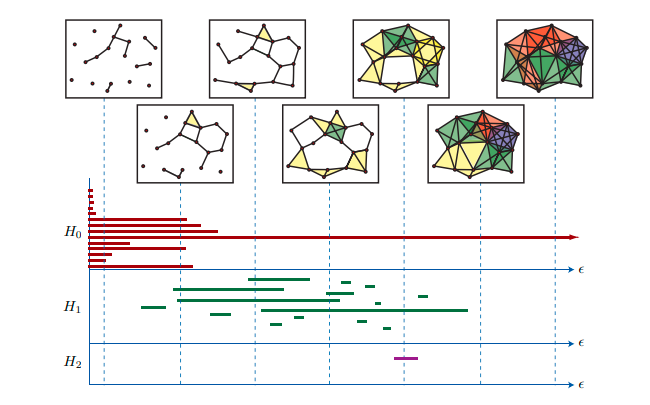
\includegraphics[width=80mm,scale=1.5]{barcodes.png}
    \caption{An example of barcode representations of the homology of the sampling of
points in an annulus }
    \label{fig:fig1}
\end{figure}
\end{frame}

  
 \subsection{Computations}
 \begin{frame}
 \begin{figure}
  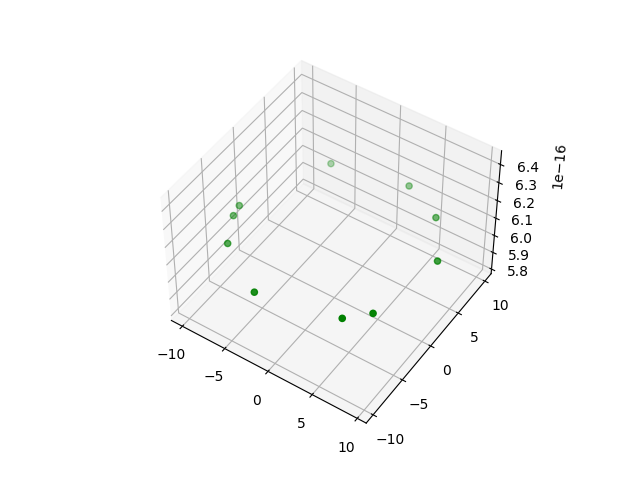
\includegraphics[width=80mm,scale=1.5]{circle.png}
    \caption{10 points on a cicle}
    \label{fig:fig1}
    \end{figure}
 \end{frame}
  
  \begin{frame}
 \begin{figure}
  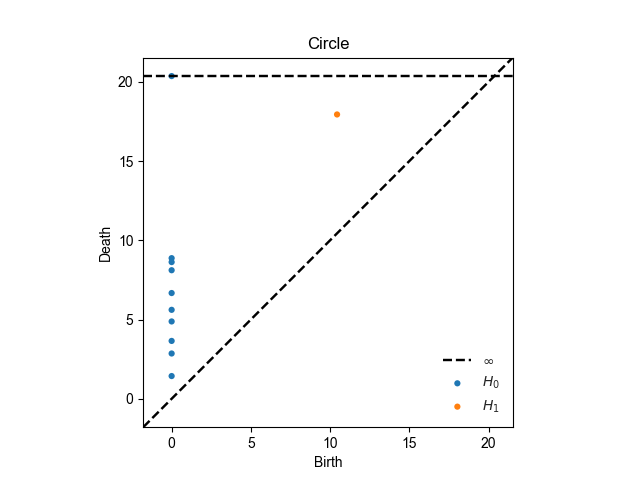
\includegraphics[width=80mm,scale=1.5]{Circle_homology.png}
    \caption{Persistent diagram of homology of circle (10 points)}
    \label{fig:fig1}
    \end{figure}
 \end{frame}
 
 \begin{frame}
 \begin{figure}
  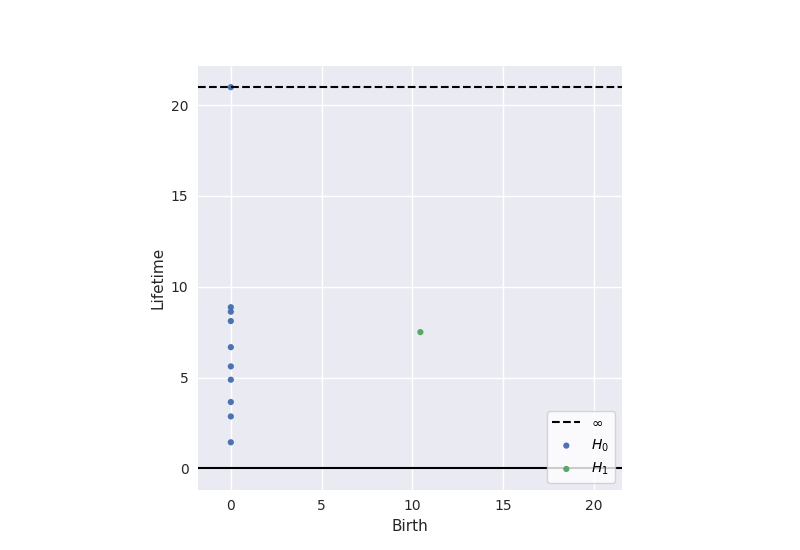
\includegraphics[width=80mm,scale=1.5]{circle_lifetime.png}
    \caption{Lifetime diagram of homology of circle (10 points)}
    \label{fig:fig1}
    \end{figure}
 \end{frame}
 
 \begin{frame}
 \begin{figure}
  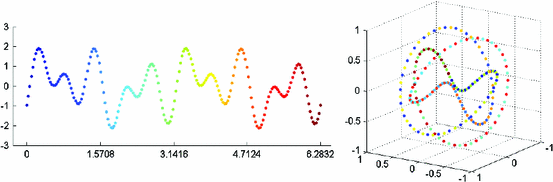
\includegraphics[width=80mm,scale=1.5]{timeseries.png}
    \caption{Peridicity in Timeseries}
    \label{fig:fig1}
    \end{figure}
 \end{frame}
 
%   \begin{frame}
%   \frametitle{References}
%   \begin{itemize}
%    \item A. Zomorodian and G. Carlsson, �Computing Persistent Homology,� Discrete Comput.
% Geom., 33, (2005), 249�274.
%    \item  A. Hatcher, Algebraic Topology, Cambridge University Press, (2002).
%    \item  V. de Silva and G. Carlsson. �Topological estimation using witness complexes,� in SPBG04
% Symposium on Point-Based Graphics (2004), 157-166
%     \item Perea, J.A., Harer, J. Sliding Windows and Persistence: An Application of Topological Methods to Signal Analysis. Found Comput Math 15, 799�838 (2015).
%     \item H. Kantz and T. Schreiber, Nonlinear Time Series Analysis, Cambridge University Press, 2003.
%     \tiem Ghrist, Robert. (2008). Barcodes: The persistent topology of data. BULLETIN (New Series) OF THE AMERICAN MATHEMATICAL SOCIETY. 45. 10.1090/S0273-0979-07-01191-3. 
%   \end{itemize}
% \end{frame}
%  
\end{document}
